\documentclass{article}
\usepackage{fullpage}
\usepackage{amsmath,amsthm,amssymb}
\usepackage{url}
\usepackage{cite}
\usepackage{xcolor,colortbl}
\usepackage{graphicx}
\usepackage{tikz}
\usetikzlibrary{chains,3d}

\newcommand{\Exp}{\text{exp}}

\begin{document}
	\hfill \textbf{Vector embeddings of time series data with linear properties}
	
	\hfill Ben Black
	
	\section{Vector embeddings}
	
	Dense data, such as images, video, and audio, is extremely high dimensional in its raw form. For many important tasks, especially information retrieval, it is extremely useful to be able to embed the important parts of the image in a vector of manageable dimension (typically on the order of 100 dimensions). Once the vectors are computed, similar images can be grouped by the similarity of their embeddings.
	
	This paper describes a new fast embedding algorithm for audio, but it can be easily generalized to other time series data. 
	
	\section{Generative vector embeddings}
	
	The idea of an embedding is taken from generative models. Take some data $A_1,A_2,A_3,...$, you want an embedding function $f$ and a decoding function $g$ such that $g(f(A_i)) \sim A_i$, where $\sim$ is some approximation relation, and the output of $f$ is smaller than the size of $A$. Then $f(A)$ is the embedding of $A$.
	
	In less mathematical terms, $f$ can be seen as a lossy compression function which compresses the data (say, a 600x800 photograph), to an embedding, say a 50 dimensional floating point vector. $g$ is the decompression function which attempts to generate an image based only on the vector. 
	
	In the deep learning paradigm, it is easy to see how to construct such an $f$ and $g$, given a $\sim$ and a dataset. It is simply to turn the approximation relation to a cost function, make $f$ and $g$ some neural network architecture, and minimize the cost of $g(f(A_i)) \sim A_i$. 
	
	The biggest problem with this model is coming up with an appropriate approximation relation $\sim$. Humans can easily tell which images are similar and different, yet when pressed, it is clear that this similarity cannot be easily described in terms of color channel magnitudes. For example, two cars, one red and one blue will have very different color channels, but humans would say that the images are quite similar compared to an image of a dog.
	
	The deep learning community's solution is adversarial networks. %In an adversarial network, after $g$ has output an image, 
	Intuitively, a generative network can be seen as a counterfitter artist, which cheaply produces images based on incomplete information about the art. The adversarial network is the authority which tries to tell counterfitted art from the real deal. In the end, we hope that the counterfitter gets better and better at producing realistic images in order to fool the authority, while the authority gets better and better and forces the counterfitter to improve even further.  
	
	More precisely, an adversarial network is a function $c$ which tries to guess whether the image $\bar{A}$ was generated by $g(f(A))$, or if it is in fact the original $A$. This adversarial network is trained separately from the generative network. 
	
	Thus, the adversarial network $c$ is attempts to optimize these two probabilities
	$$P[c(g(f(A_i))) = 0]$$
	$$P[c(A_i) = 1]$$
	It is very important that $f$ and $g$ are fixed when $c$ is training, or this would be trivially solvable. 
	
	While the generative network ($f$ and $g$) is trained to optimize the value of 
	$$P[c(g(f(A_i))) = 1]$$
	While holding $c$ fixed. 
	
	The adversarial and generative networks are then trained in an alternating sequence, so both the networks can learn from the success of the other. 
	
	
	When training is finished, remember the embedding is simply calculated by running $f(A)$, and so it can apply to data outside the original training dataset, although it is not guaranteed to generate a good embedding. 
	
	%\subsection{Problems}
	
	%Using generative vector embeddings which are constructed as described above leads to two major issues which prevent them from being used for many important purposes, including information retrieval. One is that the vectors are not guaranteed to have any substantive algebraic qualities. The other is that these models are not equipped to handle large inputs and outputs. 
	
	\subsubsection{Similarity of generative embeddings}
	
	In the classical generative embeddings described above, the embedding vector is only consumed by a single function, the decoding function $g$. Ideally, though, we want to use this vector for purposes other than applying $g$. In this paper, we will focus on using the vector for information retrieval. One important function for information retrieval is the similarity relation, which takes in two inputs and outputs a number which represents how similar the inputs are to each other. 
	
	Unfortunately, with the generative networks, there is no guarantee that classical vector similarity calculations, like squared distance or cosine distance accurately represent distance of vectors. This is because even 3 layer neural networks are universal approximators, meaning that if the network is large enough, the network can approximate any function to any degree, even highly discontinuous ones. In reality, of course, neural networks are finite and the weights are trained in a very particular way, so they do have some good properties, but we cannot a-priori say what they are. Of course, many studies have tried to fill in this gap in theory with actual results, and many of them look somewhat promising. The most promising one is the "traveling along a dimension property" (CITE case of this). However, similarity relations is not one of those promising results. This is one reason why we need a new general embedding algorithm for dense data. 
	
	\subsubsection{Large Data}
	
	Generative networks as described above have had significant success with low resolution images and audio, and more limited success with high resolution images. However, we sometimes want to get vectors of much larger data sources, for example, video. Generating more than a handful of frames of even a video would be an astronomically difficult task for a neural network, and would require enormous embeddings, and slow training. This raises the question of why we are trying to generate things in the first place if all we want is a vector. One sort of hacky solution is to average many vectors, for example make a video vector by averaging many image vectors, but averages and other cumulative methods are not likely to be good representations because of the problem with algebraic qualities mentioned above. 
	
	%Deep neural networks are functions with fixed input and output. Currently, the only well understood way of handling inputs with variable input is with recurrent networks, networks which the output of one iteration feeds into the next. The typical way of handling embeddings with these networks is to feed in the entire dataset one section at a time, and then have the network try to generate the whole dataset back, one step at a time. Unfortunately, with current state of the art (deep LSTMs), this method does not give good results for large numbers of steps (over 50 time steps). At hand here is an even 
	
	
	\section{Sparse embeddings for word2vec}
	
	One of the major advances in vector embeddings was Thomas Miktov's word2vec algorithm. This algorithm is based on the same ideas as the generative networks described above, but specialized for sequences of sparse data such as words. There are two ideas in word2vec that are critical to this work. First is to compare local context to global content, instead of generating data. Second is to rephrase the prediction problem into terms of individual vectors, instead of dense matrices. 
	
	First, lets review the basic ideas behind word2vec. The key idea behind word2vec is that the semantic meaning of a word can be described by the frequency of the words in its context. The skip-gram model leverages that by using one word in a context to try to predict other words in its context. In probabilistic terms, this means trying to estimate
	$$P[w_1 | w_2]$$ Within some specific window.  
	
	
	This model is very slow in its original form because of the softmax classification at the end. Recall that the softmax is computed by the following formula
	
	$$ \frac{\Exp(W_i x)}{\sum_j \Exp(W_j x)}$$
	In terms of the skip-gram model, $x$ would be the word vector embedding, and $W$ would be the output layer. Unfortunately, the output layer of the skip gram model scales in terms of the vocabulary size, so in order to calculate the denominator of the fraction, the algorithm needs $$(\text{vocab size}) * (\text{embedding size})$$
	Word2vec eventually solved this problem with negative sampling. The idea is to approximate the denominator by sampling a subset of the output weight vectors, instead of the entire thing. 
	$$ \frac{\Exp(W_i x)}{\sum_{j \in S} \Exp(W_j x)}$$
	$S$ is then chosen randomly from the set of words, but not uniformly: more frequent words are chosen more often than less frequent words. 
	
	These manipulations of the generative equation give rise to a completely new interpretation of what is going on:
	
	Positive sample: words $i$ and $j$ are found in the same context. Then compute $W_i O_j$.
	
	Negative sample: word $k$ is sampled randomly from the input. Compute $W_i O_k$. 
	
	Then the negative sample should have a low value as to compared to the positive sample.
	
	\section{Dense discriminative embeddings}
	
	There has been some past work on discriminative embeddings, rather than predictive embeddings. My work will follow in their footsteps. The most successful version of this is "Look, Learn, Listen" or L$^3$. These models are very powerful in the way that they say what things go where. Unfortunately, attempts to use intra-model learning through spacial reconstructions, etc have fallen far short of supervised learning techniques. \cite{DBLP:journals/corr/NorooziF16} Our goal is to have a better embedding system than them. 
	
	It is useful to see how these intra-model embeddings work. All of them try to extract high level information by using high level patterns in images. Some try to extract feature position information such as different parts of an animal by artificially creating and solving a jigsaw puzzle. Others look at frames in a video and try to extract position using match mismatch tuples. Others use gray scale to try to predict color. All of them can be termed as missing information problems. Unfortunately, the information these networks extract to solve the missing information problem never seem to be as useful a the information that supervised networks learn to find labels. 
	
	Meanwhile, other techniques, such as unsupervised learning which assumes no specific structure in the input, such as (CITE: ADVERSARIAL FEATURE LEARNING), do even worse. 
	
	Instead of hand-engineering a missing information problem, we will train the network to learn the best best possible missing information problem to solve using reinforcement learning, while solving that problem. 
	
	Another way of describing this problem is scene exploration, with the goal of finding "surprising elements" in the scene. 
	
	%But all them them try to extract high level featuring using high level patterns. 
	%Our technique is fundamentally different in all of these is that it extracts much lower level features first, and then builds upon them to form high level features. This way, nwe hope that it captures many different aspects of the image relatively well, instead of just capturing enough to solve the contrived high level problem. 
	
	
	
	\section{Algorithm}
	
	The algorithm is a neural network trying to approximate a match/mismatch problem. The match case is two local sound vector, the mismatch case is two vectors sampled uniformly from the entire dataset. 
	
	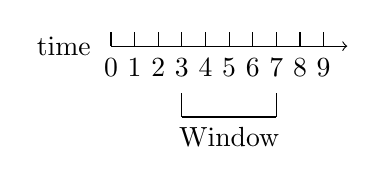
\begin{tikzpicture}[scale=0.6,mainnode/.style={font=\sffamily\footnotesize\bfseries}]
	\draw [->] (0,0) -- node[pos=-0.2] {time} (5,0);
	\foreach \tick in {0,1,2,3,4,5,6,7,8,9}
	\draw [-] (0.5*\tick,0) -- node[pos=-1.5] {\tick} (0.5*\tick,0.3);
	\draw [-] (1.5,-1) --  (1.5,-1.5);
	\draw [-] (3.5,-1) --  (3.5,-1.5);
	\draw [-] (1.5,-1.5) -- node[anchor=north] {Window} (3.5,-1.5);
	\end{tikzpicture}
	
	The mismatch case has the pair of data drawn uniformly from the entire dataset.
	
	Song ID vector
	
	\section{Results}
	
	To test the qualities of these vectors, they were \cite{DBLP:journals/corr/abs-1712-06651}
	
	
%	\begin{tikzpicture}[scale=0.6,mainnode/.style={font=\sffamily\footnotesize\bfseries}]
%	\node at (0,0) [draw] (rawdatamismatch) {Input Image};
%	\node at (3,0) [draw] (f) {$f$};
%	\node at (5,0) [draw] (embeding) {embeding};
%	\node at (8,0) [draw] (g) {$g$};
%	\node at (11,0) [draw] (genimg) {Generated image};
%	\node at (15,0) [draw] (c) {$c$};
%	\node at (16,0) [draw] (zero) {0};
%	
%	\node at (0,3) [draw] (rawdatamatch) {Input Image};
%	\node at (15,3) [draw] (cm) {$c$};
%	\node at (16,3) [draw] (zerom) {1};
%	
%	\path (rawdatamismatch)  edge node [->] {} (f);
%	\path (f)  edge node [->] {} (embeding);
%	\path (embeding)  edge node [->] {} (g);
%	\path (g)  edge node [->] {} (genimg);
%	\path (genimg)  edge node [->] {} (c);
%	\path (c)  edge node [->] {} (zero);
%	
%	\path (rawdatamatch)  edge node [->] {} (cm);
%	\path (cm)  edge node [->] {} (zerom);
%	
%	\node [fit=(rawdatamismatch)embeding)(g)(genimg),draw];
%	\end{tikzpicture}
	
%	\begin{tikzpicture}
%	%\draw[->] (0,0,0) -- node[pos=1.2] {x} (1,0,0);
%	%\draw[->] (0,0,0) -- node[pos=1.2] {y} (0,1,0);
%	%\draw[->] (0,0,0) -- node[pos=1.2] {z} (0,0,1);
%	
%	\draw[->] (0,0,0) -- node[anchor=north] {28} (0,0,5);
%	\draw[->] (0,0,0) -- node[anchor=west] {28} (0,5,0);
%	%\draw[->] (0,0,0) -- node[pos=1.2] {28} (0,0,5);
%	\fill[blue!50,opacity=0.6,canvas is yz plane at x=0,draw=black] (0,0) rectangle (5,5);
%	
%	\draw[->] (0.5,2,2) -- node [anchor=north] {5} (0.5,2,3);
%	\draw[->] (0.5,2,2) -- node [anchor=west] {5} (0.5,3,2);
%	\fill[red!50,opacity=0.6,canvas is yz plane at x=0.5,draw=black] (2,2) rectangle (3,3);
%	
%	%\draw [step=0.3cm] [blue!50,opacity=0.6,draw=black] (0,0,0) -- (0,0,5) -- (0,5,5) -- (0,5,0);
%	
%	\end{tikzpicture}
	
	
	
	\bibliography{linearlizer_rewrite}{}
	\bibliographystyle{plain}
	
\end{document}